\documentclass[12pt,a4paper]{report}

% -------------------------------------------------------------------------
% PACKAGES
% -------------------------------------------------------------------------
\usepackage[utf8]{inputenc}
\usepackage[T1]{fontenc}
\usepackage{lmodern}
\usepackage[a4paper, margin=1in, top=1.2in, bottom=1.2in]{geometry}
\usepackage{graphicx}
\usepackage{amsmath, amssymb}
\usepackage{booktabs}
\usepackage{float}
\usepackage{array}
\usepackage{titlesec}
\usepackage{fancyhdr}
\usepackage{hyperref}
\usepackage{tikz}
\usetikzlibrary{shapes.geometric, arrows.meta, positioning, fit, calc}

% -------------------------------------------------------------------------
% HYPERLINK SETUP
% -------------------------------------------------------------------------
\hypersetup{
    colorlinks=true,
    linkcolor=black,
    citecolor=black,
    urlcolor=blue
}

% -------------------------------------------------------------------------
% HEADER & FOOTER
% -------------------------------------------------------------------------
\pagestyle{fancy}
\fancyhf{}
\fancyhead[L]{\small Skill Connect}
\fancyhead[R]{\small Seminar-I}
\fancyfoot[C]{\thepage}
\renewcommand{\headrulewidth}{0.4pt}
\renewcommand{\footrulewidth}{0pt}

% -------------------------------------------------------------------------
% SECTION FORMATTING (Matches Friend's Inline Chapter Title Format)
% -------------------------------------------------------------------------
\titleformat{\chapter}[hang]
  {\normalfont\LARGE\bfseries}
  {Chapter \thechapter\quad}
  {0pt}
  {\LARGE\bfseries}

\titlespacing*{\chapter}{0pt}{20pt}{20pt}
\titlespacing*{\section}{0pt}{14pt}{8pt}
\titlespacing*{\subsection}{0pt}{10pt}{6pt}

\setlength{\parindent}{1.5em}
\setlength{\parskip}{0.4em}
\linespread{1.18}

% -------------------------------------------------------------------------
% PROJECT METADATA (Customizable)
% -------------------------------------------------------------------------
\newcommand{\ProjectTitle}{SKILL CONNECT}
\newcommand{\ProjectSubtitle}{A Campus Peer-to-Peer Skill Exchange and Learning Network}
\newcommand{\UniversityName}{SANJIVANI UNIVERSITY}
\newcommand{\SchoolName}{School of Engineering and Technology}
\newcommand{\DepartmentName}{Department of Computer Science and Engineering}

% Student details
\newcommand{\StudentOne}{Mahesh Bangar -- 2125UCEM1012}
\newcommand{\StudentTwo}{Saksham Patil -- 2125UCEM1034}
\newcommand{\StudentThree}{Saisha Asane -- 2125UCEF1015}
\newcommand{\StudentFour}{Chandana Bothara -- 2125UCEF1051}

\newcommand{\GuideName}{Prof. Jyotimoyee Kalita}
\newcommand{\HODName}{Dr. Mahendra Gawali}
\newcommand{\AcademicYear}{2026--2027}

% =========================================================================
\begin{document}
% =========================================================================

% -------------------------------------------------------------------------
% TITLE PAGE
% -------------------------------------------------------------------------
\begin{titlepage}
\thispagestyle{empty}
\centering

{\textbf{\LARGE \UniversityName}\par}
\vspace{0.25cm}
{\textbf{\large \SchoolName}\par}
\vspace{0.15cm}
{\DepartmentName\par}

\vfill
{\textbf{\large SEMINAR-I PROJECT REPORT}\par}

\vfill
{\textbf{\huge \ProjectTitle}\par}
\vspace{0.35cm}
{\textbf{\large \ProjectSubtitle}\par}

\vfill
{\small Submitted By\par}
\vspace{0.35cm}
{\StudentOne\par}
\vspace{0.15cm}
{\StudentTwo\par}
\vspace{0.15cm}
{\StudentThree\par}
\vspace{0.15cm}
{\StudentFour\par}

\vfill
{\small Under the Guidance of\par}
\vspace{0.35cm}
{\textbf{\large \GuideName}\par}

\vfill
{Subject: Seminar-I\par}
\vspace{0.15cm}
{Academic Year: \AcademicYear\par}

\vspace{0.8cm}
{\textbf{Head of Department}\par}
\vspace{0.15cm}
{\HODName\par}

\end{titlepage}

% -------------------------------------------------------------------------
% ABSTRACT
% -------------------------------------------------------------------------
\newpage
\pagenumbering{arabic}
\setcounter{page}{1}

\section*{Abstract}
\addcontentsline{toc}{chapter}{Abstract}

Higher education campuses bring together diverse cohorts of students possessing varied technical specializations, creative proficiencies, and interpersonal skills. However, peer knowledge sharing on campus remains largely fragmented and serendipitous. Students seeking practical mentorship in modern domains---such as machine learning, web engineering, UI/UX design, or public speaking---frequently struggle to locate suitable peer partners within their university ecosystem. Conversely, skilled students lack a structured, credit-free channel to share their knowledge and gain reciprocal learning opportunities.

Skill Connect is a campus-focused peer-to-peer skill exchange platform engineered to facilitate direct, reciprocal learning within university communities. Operating on a mutual skill-barter model, the system enables students to declare competencies they can teach alongside topics they aspire to learn. The platform features verified campus authentication, an onboarding wizard, an algorithmic peer-matching engine, interest-based campus circles, scheduled peer sessions with interactive calendar synchronization, real-time peer messaging, dynamic skill demand polling, and a global search command palette.

The project follows a structured modular engineering methodology spanning requirement analysis, user research, architectural design, component-driven UI/UX development, reactive client-side state persistence, and verification. Currently, the platform has completed advanced frontend development and integration, validating core user workflows, responsive interfaces, and client-side data persistence.

The remaining work mainly focuses on final validation, refinement, and preparation for deployment and demonstration. Future scope explores extensions such as real-time audio/video peer classrooms, cryptographic tokenized skill endorsements, automated attendance verification via dynamic QR tokens, and inter-university cross-campus collaborative networks.

\vspace{1cm}
\noindent\textbf{Keywords:} Peer-to-Peer Learning, Skill Barter, Campus Network, Intelligent Matching, Collaborative Education, React Architecture.

% -------------------------------------------------------------------------
% TABLE OF CONTENTS
% -------------------------------------------------------------------------
\newpage
\tableofcontents

% -------------------------------------------------------------------------
% LIST OF FIGURES & TABLES
% -------------------------------------------------------------------------
\newpage
\listoffigures

\newpage
\listoftables

% =========================================================================
% CHAPTER 1: INTRODUCTION
% =========================================================================
\newpage
\chapter{Introduction}

\section{Background}
University ecosystems represent dense knowledge hubs where thousands of students concurrently pursue academic and professional growth. Outside of standardized lecture curricula, students acquire specialized competencies ranging from coding frameworks, machine learning, and cloud infrastructure to non-technical proficiencies such as graphic design, photography, leadership, and interview readiness.

Despite this abundance of campus talent, students seeking hands-on mentorship often find it difficult to identify suitable peers. Traditional mechanisms for extracurricular learning rely heavily on informal WhatsApp groups, social networks, or student club announcements. These informal channels are unstructured, noisy, unindexed, and lack verified accountability. Consequently, knowledge remains siloed within immediate friend groups or isolated academic branches.

Digital technology offers a viable framework to organize and democratize peer learning. A centralized, campus-dedicated digital platform can catalog student skill competencies, compute complementary learning pairs, coordinate scheduled learning sessions, and foster continuous community interactions without financial barriers.

Skill Connect is conceived around this principle: transforming an entire university campus into an interconnected, decentralized learning network where every student is simultaneously a teacher and a learner.

\section{Motivation}
The main motivation behind Skill Connect is the difficulty students face when trying to find peer collaborators, practical mentors, and relevant skill resources across disconnected campus groups.

In typical campus environments, a third-year computer science student proficient in Python may want to learn UI/UX design, while a design or electronics student possessing strong Figma skills desires guidance in programming fundamentals. Currently, no unified platform programmatically matches these inverse learning needs. Students either resort to expensive third-party online courses that lack personalized feedback, or miss collaborative opportunities altogether.

Furthermore, students who teach reinforce their own mastery through active pedagogical practice, known as the Prot\'eg\'e Effect. Skill Connect eliminates commercialization by establishing a pure reciprocal barter economy: knowledge is exchanged for knowledge, fostering egalitarian campus collaboration.

\section{Project Vision}
The vision of Skill Connect is to provide a simple, intuitive, and well-organized digital platform that can connect students with campus-wide learning and skill-sharing opportunities.

The platform is not intended to replace university professors, lectures, or formal academic curricula. Instead, it is designed to make the process of finding peer mentors, collaborating across departments, and organizing informal study sessions significantly more structured and accessible.

\section{Scope of the Project}
The main modules planned and developed for the platform comprise:
\begin{itemize}
    \setlength{\itemsep}{1.5pt}
    \setlength{\parskip}{0pt}
    \item User Login and Role-Aware Authentication
    \item Multi-Step Onboarding and Profile Setup Wizard
    \item Main Dashboard and Skill Snapshot Analytics
    \item Smart Peer Matching and Discovery
    \item Campus Circles (Communities) and Discussions
    \item Peer Learning Sessions and RSVP Management
    \item Interactive Calendar
    \item Real-Time Peer Messaging and Chat
    \item Campus Skill Demand Polls
    \item Global Command Palette (\textbf{Cmd+K} Search Overlay)
    \item Profile Customization and Skill Barter Management
\end{itemize}

The project has progressed through the initial design and development stages and is currently in the advanced integration, testing, and refinement stage. The frontend components and local storage state persistence have been brought together for comprehensive functional validation.

% =========================================================================
% CHAPTER 2: PROBLEM STATEMENT, OBJECTIVES AND SCOPE
% =========================================================================
\newpage
\chapter{Problem Statement, Objectives and Scope}

\section{Problem Statement}
Students in higher education institutions frequently encounter challenges when seeking peer mentors, organizing collaborative study sessions, and identifying classmates with complementary skill sets.

In many situations, these activities are handled through fragmented channels such as scattered messaging groups, individual verbal requests, social media, or departmental noticeboards. This makes peer discovery unorganized, serendipitous, and time-consuming.

Existing educational platforms often focus exclusively on formal coursework, commercial tutoring, or general professional networking, leaving a notable gap for a dedicated campus-bounded peer skill exchange platform.

Based on these challenges, the problem addressed by this project is:
\begin{quote}
\textit{How can campus skill competencies and learning needs be organized in one simple, responsive digital platform that enables reciprocal peer matching and collaborative knowledge exchange for university students?}
\end{quote}

\section{Objectives}
The main objectives of Skill Connect are:
\begin{enumerate}
    \item To provide a single, dedicated campus platform for accessing peer-to-peer learning and skill-sharing services.
    \item To implement a guided onboarding workflow that captures student identities, skills they can teach, and skills they want to learn.
    \item To compute complementary peer matches based on reciprocal skill alignment.
    \item To provide domain-specific campus circles for collaborative learning and discussions.
    \item To provide a structured session creation and seat reservation process.
    \item To integrate an interactive calendar for tracking scheduled peer sessions.
    \item To provide a peer messaging interface for direct communication.
    \item To incorporate campus-wide skill demand polls to identify high-interest learning topics.
    \item To provide an omnipresent search overlay with keyboard shortcuts (\textbf{Cmd+K}) for quick navigation.
    \item To develop a responsive, modern interface with dual light and dark theme support.
\end{enumerate}

\section{Expected Outcome}
The current outcome of the project is a near-complete working system that demonstrates the major functions and overall user flow of the application.

The project is currently in its final integration and validation stage, with the frontend components, custom router, and reactive state management brought together so that student profiles, skills, sessions, communities, messages, and poll votes are dynamically managed and persisted.

% =========================================================================
% CHAPTER 3: LITERATURE REVIEW AND RESEARCH GAP
% =========================================================================
\newpage
\chapter{Literature Review and Research Gap}

\section{Peer-to-Peer Collaborative Learning}
Collaborative and peer-led learning has long been recognized in pedagogical research as an effective methodology for deep understanding and knowledge retention. According to Topping \cite{topping2005trends}, peer learning allows students to interact in cognitively congruent ways, communicating difficult technical ideas using relatable language and shared academic contexts.

Furthermore, educational psychology studies show that teaching peers fosters the Prot\'eg\'e Effect, where students who prepare to teach others demonstrate higher conceptual clarity, metacognitive monitoring, and long-term retention compared to passive learners \cite{nestojko2014expecting}. Skill Connect operationalizes this dynamic by structuring learning around mutual exchange.

\section{Digital Learning Networks on Campuses}
Learning Management Systems (LMS) such as Moodle and Blackboard are standard across universities, yet studies by Dahlstrom et al. \cite{dahlstrom2014study} highlight that students view traditional LMS platforms primarily as administrative repositories for grades and syllabus files, rather than vibrant spaces for student-to-student collaboration.

Informal communication frequently migrates to social messaging applications such as WhatsApp and Telegram. However, research into educational social media usage demonstrates that unindexed chat streams suffer from cognitive overload, lack of searchability, and absence of formal scheduling tools \cite{tang2017students}.

\section{Skill Matching and Taxonomy Systems}
The effectiveness of knowledge-sharing networks relies on structured categorization and matchmaking algorithms. Recommender systems literature by Resnick and Varian \cite{resnick1997recommender} outlines collaborative filtering and bipartite matching heuristics, where the mutual alignment of two parties' needs and capabilities yields optimal collaborative engagement.

In Skill Connect, this heuristic is adapted into a campus taxonomy separating technical proficiencies (such as Python, Java, Web Development, and AI/ML) from human proficiencies (such as Public Speaking, Photography, and Content Creation), enabling precise multi-attribute peer discovery.

\section{Micro-Mentorship and Collaborative Scheduling}
Micro-mentorship involves brief, targeted, low-stakes knowledge-sharing interactions rather than prolonged formal commitments. Gale et al. \cite{gale2020micro} observed that micro-mentorship lowers the barrier for undergraduate participation and significantly increases inter-disciplinary engagement.

A core bottleneck identified in academic mentoring is scheduling friction. Introducing structured session booking with explicit capacity controls and date-mapped calendar views directly mitigates these organizational drop-offs.

\section{Research Gap}
Existing platforms present clear limitations when applied to undergraduate campus peer learning:
\begin{itemize}
    \item Commercial course platforms (Coursera, Udemy) provide one-way video lectures with no personalized peer assistance.
    \item Commercial tutoring marketplaces (Chegg, Preply) require financial transactions, making them inaccessible to typical students.
    \item Professional networks (LinkedIn) focus on external career resumes rather than informal campus study groups.
    \item Campus forums (Reddit, Discord) lack structured identity verification, availability tracking, and calendar booking.
\end{itemize}

There is a distinct opportunity to combine profile verification, reciprocal skill matching, community circles, session scheduling, calendar visualization, and live peer messaging into a single, cohesive campus platform. Skill Connect addresses this gap directly.

% =========================================================================
% CHAPTER 4: PROPOSED METHODOLOGY
% =========================================================================
\newpage
\chapter{Proposed Methodology}

\section{Overview}
The project has been developed in multiple stages instead of building all the modules at once. This made it easier for the team to divide the work, test individual modules, and integrate them systematically. The project is now in the final integration, testing, and refinement stage.

The overall methodology is:
\begin{quote}
\centering
Requirement Analysis $\longrightarrow$ Research $\longrightarrow$ System Design $\longrightarrow$ UI/UX Design $\longrightarrow$ Frontend Development $\longrightarrow$ State Modeling \& Persistence $\longrightarrow$ Integration $\longrightarrow$ Testing
\end{quote}

\section{Requirement Analysis}
The first step was to identify the main problems that the platform should address within our university environment. The requirements identified for the application include:
\begin{itemize}
    \item User login with institutional email validation and demo access
    \item Multi-step onboarding to capture name, department, bio, skills, and availability
    \item Campus dashboard showing personal skill metrics and recommended peers
    \item Smart matching matrix displaying reciprocal match percentages
    \item Campus circles for topical community discussions
    \item Workshop session booking with seat capacity management
    \item August monthly calendar with session mapping
    \item Peer-to-peer direct messaging interface
    \item Campus skill demand polling
    \item Quick search command palette (\textbf{Cmd+K})
    \item Profile editor allowing updates to bio, skills, and community memberships
\end{itemize}

\section{Research}
Research was carried out on campus learning habits, collaborative filtering techniques, peer-to-peer knowledge exchange platforms, and usability in student applications.

The research helped us understand that the platform should not only focus on listing skills. Usability factors such as clean typography, dual-theme support, rapid keyboard navigation, clear error indicators, and persistent state across page reloads are essential for everyday student adoption.

\section{System Design}
After identifying the requirements, the system was divided into modular functional components:
\begin{enumerate}
    \item Login Module
    \item Onboarding Module
    \item Dashboard Module
    \item Explore Module
    \item Matches Module
    \item Communities Module
    \item Community Detail Module
    \item Sessions Module
    \item Calendar Module
    \item Chat Module
    \item Polls Module
    \item Search Overlay Module
    \item Profile Module
    \item Settings Module
\end{enumerate}

This modular approach allows individual components to be developed, styled, and validated independently while maintaining a cohesive look and feel.

\section{UI/UX Design}
The interface was designed with a modern, high-contrast, campus-centric look in mind. The design utilizes card containers, rounded borders, clear typographic hierarchy, consistent spacing, and an accent indigo theme color (\texttt{\#6254dc}).

A reusable CSS architecture was created using custom CSS properties in \texttt{styles.css} and \texttt{refinement.css}. This enables automatic theming (Light and Dark modes) and ensures uniform padding, border-radius, and typography across all pages.

\section{Frontend Development}
The frontend has been developed using:
\begin{itemize}
    \item \textbf{HTML5}: Semantic page structure and accessible forms.
    \item \textbf{CSS3}: Modular design tokens, custom properties, Flexbox, and CSS Grid layouts.
    \item \textbf{JavaScript (ES2022)}: Client-side reactive logic and data handling.
    \item \textbf{React 19}: Component-based architecture and state hooks (\texttt{useState}, \texttt{useEffect}, \texttt{useMemo}, \texttt{useRef}).
    \item \textbf{Vite 8.2}: High-speed bundler and local development environment.
    \item \textbf{Lucide React}: Clean, uniform SVG icons.
\end{itemize}

\section{State Architecture and Persistence}
To deliver a fully functioning application without initial server dependencies, client-side persistence is implemented via a custom \texttt{usePersisted} hook that mirrors state into browser \texttt{localStorage}. This guarantees that student profiles, registered sessions, joined communities, poll votes, and notifications persist across browser refreshes.

\section{Backend and Database Design (Future Scope)}
The planned backend follows a RESTful microservice model using Node.js/Express or Java Spring Boot connected to a relational MySQL/PostgreSQL database.
Major entities include:
\begin{itemize}
    \item \textbf{Users}: ID, name, email, department, year, bio, availability mode
    \item \textbf{Skills}: ID, name, category (Technical, Non-Technical)
    \item \textbf{UserSkills}: User ID, Skill ID, type (Teach, Learn)
    \item \textbf{Communities}: ID, name, topic, category, member count
    \item \textbf{Sessions}: ID, skill name, host name, date, time, mode, venue, seats, capacity
    \item \textbf{Messages}: ID, sender ID, recipient ID, text, timestamp
    \item \textbf{PollVotes}: Poll ID, option index, user ID
\end{itemize}

\section{Integration and Testing}
Frontend components communicate through central application state passed via route shells. Testing was conducted alongside development, covering functional test cases, form validation, theme switching, responsive viewports, and keyboard shortcut event listeners.

\newpage
\section{System Workflow}
The overall workflow of Skill Connect begins when a student opens the application and signs in or continues as a demo user. If the student has not completed onboarding, they are routed to the 4-step profile setup wizard. Once completed, the student accesses the main dashboard, which serves as the hub for exploring skills, discovering matched peers, joining communities, registering for sessions, chatting, and voting on campus polls.

The system workflow is shown in Figure \ref{fig:workflow}.

\begin{figure}[htbp]
\centering
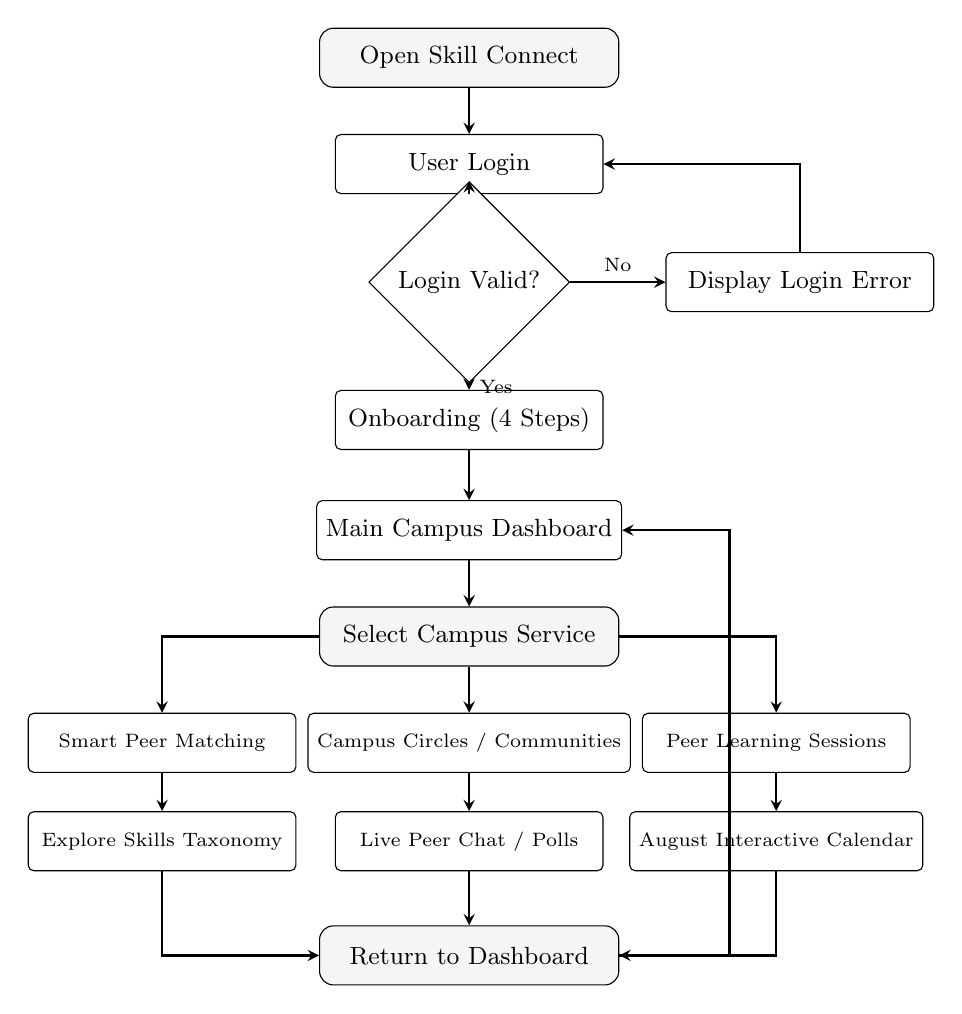
\begin{tikzpicture}[
    auto,
    startstop/.style={rectangle, rounded corners=5pt, minimum width=3.8cm, minimum height=0.75cm, text centered, draw=black, fill=gray!8, font=\small},
    process/.style={rectangle, rounded corners=2pt, minimum width=3.4cm, minimum height=0.75cm, text centered, draw=black, fill=white, font=\small},
    decision/.style={diamond, minimum width=2.4cm, minimum height=1.1cm, text centered, draw=black, fill=white, font=\small},
    modbox/.style={rectangle, rounded corners=2pt, minimum width=3.4cm, minimum height=0.75cm, text centered, draw=black, fill=white, font=\scriptsize},
    arrow/.style={thick, ->, >=stealth}
]

% Main Spine
\node (open) [startstop] {Open Skill Connect};
\node (login) [process, below of=open, yshift=-0.35cm] {User Login};
\node (check) [decision, below of=login, yshift=-0.5cm] {Login Valid?};
\node (err) [process, right of=check, xshift=3.2cm] {Display Login Error};
\node (onboard) [process, below of=check, yshift=-0.75cm] {Onboarding (4 Steps)};
\node (dash) [process, below of=onboard, yshift=-0.4cm] {Main Campus Dashboard};
\node (select) [startstop, below of=dash, yshift=-0.35cm] {Select Campus Service};

% 3 Parallel Columns (Identical to reference report layout)
\node (m_col2) [modbox, below of=select, yshift=-0.35cm] {Campus Circles / Communities};
\node (m_col1) [modbox, left of=m_col2, xshift=-2.9cm] {Smart Peer Matching};
\node (m_col3) [modbox, right of=m_col2, xshift=2.9cm] {Peer Learning Sessions};

\node (s_col2) [modbox, below of=m_col2, yshift=-0.25cm] {Live Peer Chat / Polls};
\node (s_col1) [modbox, below of=m_col1, yshift=-0.25cm] {Explore Skills Taxonomy};
\node (s_col3) [modbox, below of=m_col3, yshift=-0.25cm] {August Interactive Calendar};

% Return
\node (return) [startstop, below of=s_col2, yshift=-0.45cm] {Return to Dashboard};

% Clean non-intersecting connectors
\draw [arrow] (open) -- (login);
\draw [arrow] (login) -- (check);
\draw [arrow] (check) -- node[above, font=\scriptsize] {No} (err);
\draw [arrow] (err) |- (login);
\draw [arrow] (check) -- node[right, font=\scriptsize] {Yes} (onboard);
\draw [arrow] (onboard) -- (dash);
\draw [arrow] (dash) -- (select);

% Fan out to 3 columns
\draw [arrow] (select) -| (m_col1);
\draw [arrow] (select) -- (m_col2);
\draw [arrow] (select) -| (m_col3);

\draw [arrow] (m_col1) -- (s_col1);
\draw [arrow] (m_col2) -- (s_col2);
\draw [arrow] (m_col3) -- (s_col3);

\draw [arrow] (s_col1) |- (return);
\draw [arrow] (s_col2) -- (return);
\draw [arrow] (s_col3) |- (return);

% Clean right-side return loop back to Dashboard
\draw [arrow] (return.east) -- ++(1.4cm,0) |- (dash.east);
\end{tikzpicture}
\caption{Skill Connect System Workflow}
\label{fig:workflow}
\end{figure}

\newpage
\section{System Architecture}
Skill Connect follows a layered architecture where presentation, client-side application logic, and persistence are kept as separate layers. This makes the application clean, responsive, and ready for future database connectivity.

The system architecture is shown in Figure \ref{fig:architecture}.

\begin{figure}[htbp]
\centering
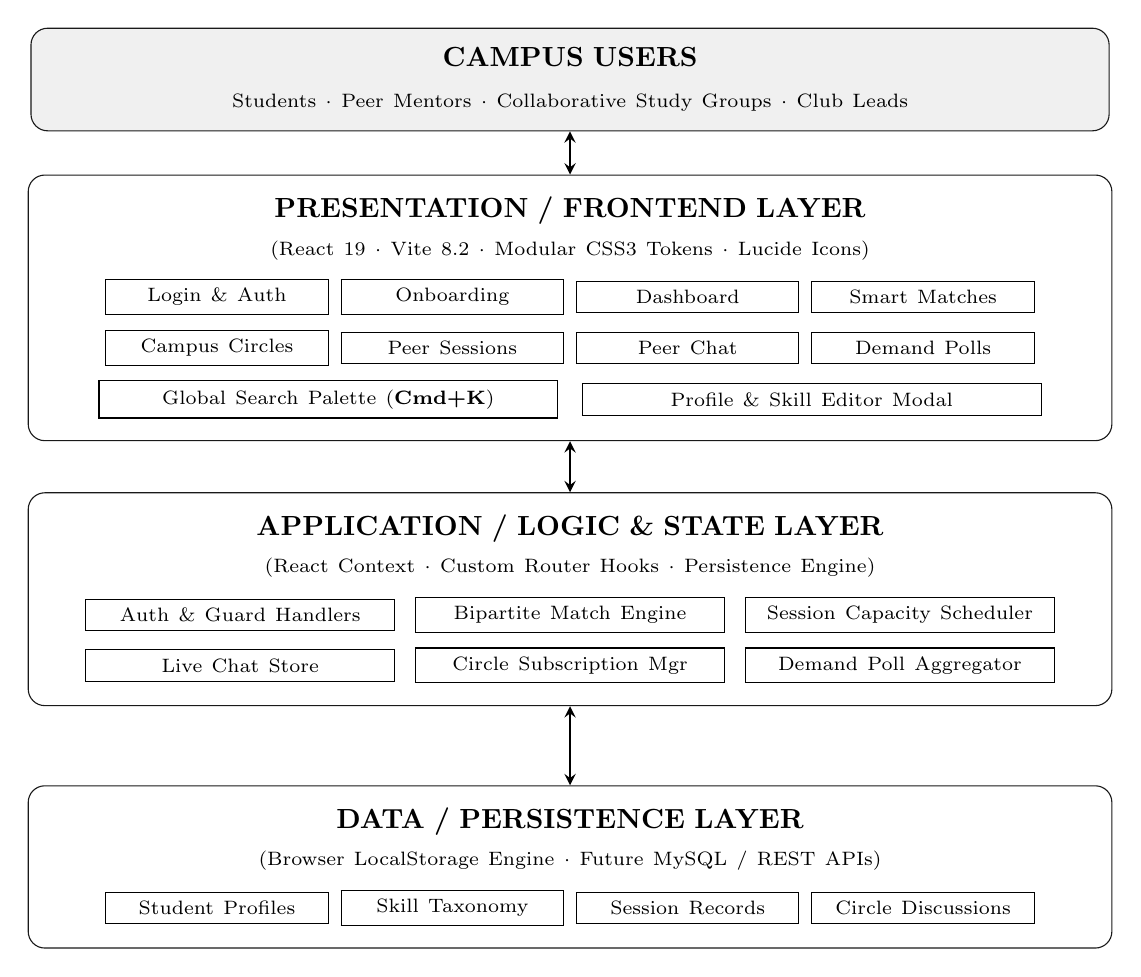
\begin{tikzpicture}[
    every node/.style={align=center},
    userbox/.style={rectangle, rounded corners=6pt, draw=black!90, fill=gray!12, text width=13.2cm, inner sep=7pt, align=center},
    layerbox/.style={rectangle, rounded corners=6pt, draw=black!90, fill=white, text width=13.2cm, inner sep=8pt, align=center},
    arrow/.style={thick, <->, >=stealth}
]

% User Layer
\node (user) [userbox] {
    \textbf{CAMPUS USERS}\\[0.1cm]
    \scriptsize Students $\cdot$ Peer Mentors $\cdot$ Collaborative Study Groups $\cdot$ Club Leads
};

% Presentation Layer
\node (pres) [layerbox, below of=user, yshift=-1.9cm] {
    \textbf{PRESENTATION / FRONTEND LAYER}\\[0.05cm]
    {\scriptsize (React 19 $\cdot$ Vite 8.2 $\cdot$ Modular CSS3 Tokens $\cdot$ Lucide Icons)}\\[0.2cm]
    \fbox{\parbox{2.6cm}{\centering\scriptsize Login \& Auth}}\hspace{0.15cm}%
    \fbox{\parbox{2.6cm}{\centering\scriptsize Onboarding}}\hspace{0.15cm}%
    \fbox{\parbox{2.6cm}{\centering\scriptsize Dashboard}}\hspace{0.15cm}%
    \fbox{\parbox{2.6cm}{\centering\scriptsize Smart Matches}}\\[0.15cm]
    \fbox{\parbox{2.6cm}{\centering\scriptsize Campus Circles}}\hspace{0.15cm}%
    \fbox{\parbox{2.6cm}{\centering\scriptsize Peer Sessions}}\hspace{0.15cm}%
    \fbox{\parbox{2.6cm}{\centering\scriptsize Peer Chat}}\hspace{0.15cm}%
    \fbox{\parbox{2.6cm}{\centering\scriptsize Demand Polls}}\\[0.15cm]
    \fbox{\parbox{5.6cm}{\centering\scriptsize Global Search Palette (\textbf{Cmd+K})}}\hspace{0.3cm}%
    \fbox{\parbox{5.6cm}{\centering\scriptsize Profile \& Skill Editor Modal}}
};

% Application Layer
\node (app) [layerbox, below of=pres, yshift=-2.7cm] {
    \textbf{APPLICATION / LOGIC \& STATE LAYER}\\[0.05cm]
    {\scriptsize (React Context $\cdot$ Custom Router Hooks $\cdot$ Persistence Engine)}\\[0.2cm]
    \fbox{\parbox{3.7cm}{\centering\scriptsize Auth \& Guard Handlers}}\hspace{0.25cm}%
    \fbox{\parbox{3.7cm}{\centering\scriptsize Bipartite Match Engine}}\hspace{0.25cm}%
    \fbox{\parbox{3.7cm}{\centering\scriptsize Session Capacity Scheduler}}\\[0.15cm]
    \fbox{\parbox{3.7cm}{\centering\scriptsize Live Chat Store}}\hspace{0.25cm}%
    \fbox{\parbox{3.7cm}{\centering\scriptsize Circle Subscription Mgr}}\hspace{0.25cm}%
    \fbox{\parbox{3.7cm}{\centering\scriptsize Demand Poll Aggregator}}
};

% Data Layer
\node (data) [layerbox, below of=app, yshift=-2.4cm] {
    \textbf{DATA / PERSISTENCE LAYER}\\[0.05cm]
    {\scriptsize (Browser LocalStorage Engine $\cdot$ Future MySQL / REST APIs)}\\[0.2cm]
    \fbox{\parbox{2.6cm}{\centering\scriptsize Student Profiles}}\hspace{0.15cm}%
    \fbox{\parbox{2.6cm}{\centering\scriptsize Skill Taxonomy}}\hspace{0.15cm}%
    \fbox{\parbox{2.6cm}{\centering\scriptsize Session Records}}\hspace{0.15cm}%
    \fbox{\parbox{2.6cm}{\centering\scriptsize Circle Discussions}}
};

% Layer Connectors
\draw [arrow] (user) -- (pres);
\draw [arrow] (pres) -- (app);
\draw [arrow] (app) -- (data);

\end{tikzpicture}
\caption{System Architecture of Skill Connect}
\label{fig:architecture}
\end{figure}

% =========================================================================
% CHAPTER 5: IMPLEMENTATION
% =========================================================================
\newpage
\chapter{Implementation}

\section{Current Implementation}
The frontend has been developed module by module using the common CSS architecture created for the project and is currently undergoing final integration and refinement.

The completed modules currently include:
\begin{itemize}
    \item Login Module
    \item Onboarding Module
    \item Dashboard Module
    \item Smart Peer Matching Module
    \item Campus Circles (Communities) Module
    \item Peer Learning Sessions Module
    \item August Calendar Module
    \item Real-Time Chat Module
    \item Demand Polls Module
    \item Global Search Overlay (\textbf{Cmd+K})
    \item Profile and Skills Customizer Modal
\end{itemize}

\section{Login Module}
The Login page provides the initial entry point for the user.
It contains:
\begin{itemize}
    \item College email field
    \item Password field
    \item Inline field error validation
    \item Sign In action button
    \item ``Continue as Demo Student'' action which safely re-initializes an un-onboarded profile and transitions into the Onboarding wizard
\end{itemize}

\section{Onboarding Module}
The Onboarding module collects essential student attributes through a guided 4-step form:
\begin{itemize}
    \item \textbf{Step 1 (Profile Info)}: Collects student name, academic department, and a short bio. Enforces non-empty name validation.
    \item \textbf{Step 2 (What can you teach?)}: Chip-selector for choosing technical skills (Python, Web Dev, Java, AI/ML, Cloud) and non-technical skills (Public Speaking, Photography, UI/UX). Requires at least 1 selection.
    \item \textbf{Step 3 (What do you want to learn?)}: Chip-selector for defining desired learning topics. Requires at least 1 selection.
    \item \textbf{Step 4 (Availability)}: Preference selector for Online, Offline, or Both.
    \item \textbf{Completion}: Generates student avatar initials and redirects to the dashboard with a welcome confirmation.
\end{itemize}

\section{Dashboard Module}
The Dashboard is the main page after login.
It includes:
\begin{itemize}
    \item Welcome header with active campus student status indicator
    \item Skill Snapshot showing counts of teachable skills, target learning skills, and technical/human balance
    \item Big search button triggering the global command palette
    \item Top matched peer recommendations
    \item Upcoming learning session preview
    \item Campus Pulse trending skill charts
    \item Subscribed communities carousel
\end{itemize}

\section{Smart Matching Module}
The Matches page connects students with complementary learning goals.
Features include:
\begin{itemize}
    \item Filter chips: \textit{Best Match}, \textit{Technical}, \textit{Non-Technical}, \textit{Online}, \textit{Offline}
    \item Peer match cards displaying match percentage, department, year, can-teach chips, and wants-to-learn chips
    \item Direct ``Connect'' action triggering toast confirmation
    \item Link to view peer's full profile
\end{itemize}

\section{Campus Circles Module}
The Communities page enables topic-based interaction.
It features:
\begin{itemize}
    \item Categorized circle grids (Technical and Non-Technical)
    \item Community cards displaying member count, online count, trending topics, and 1-click Join/Leave toggles
    \item Community Detail view containing overview discussions, active peer members, and upcoming circle workshops
\end{itemize}

\section{Peer Learning Sessions and Calendar Module}
This module handles workshop organization:
\begin{itemize}
    \item Lists upcoming sessions with date, time, mentor name, mode (Online/Offline), and available seats
    \item Modal dialog allowing students to create and schedule new sessions
    \item \textbf{Interactive Calendar}: Visual August 2026 grid marking dates with active sessions, allowing students to inspect time, location, and mentor information by clicking on any date
\end{itemize}

\section{Chat Module}
The Chat module provides a direct messaging interface:
\begin{itemize}
    \item Sidebar listing recent peer conversations with presence indicators
    \item Active chat window displaying sent and received message bubbles with timestamps
    \item Real-time message submission with immediate feedback
\end{itemize}

\section{Campus Demand Polls Module}
The Polls page facilitates collective decision-making:
\begin{itemize}
    \item Open poll where students vote on which skill workshop should be scheduled next
    \item Dynamic percentage fill meters indicating real-time student demand
    \item Single-vote locking mechanism preventing ballot stuffing
\end{itemize}

\section{Global Command Palette and Search Overlay}
The platform provides a centralized search overlay:
\begin{itemize}
    \item Accessible via clicking topbar/dashboard search buttons or pressing \textbf{Cmd+K} / $\mathbf{Ctrl+K}$
    \item Instant live filtering across Students, Communities, and Skills
    \item Direct keyboard navigation and $\mathbf{Escape}$ dismissal
\end{itemize}

\section{Profile Customizer Module}
The Profile page enables comprehensive self-management:
\begin{itemize}
    \item Renders student avatar, department, bio, badges, rating, and sessions completed
    \item Multi-tab modal editor allowing students to update their bio, toggle teaching skills, toggle learning goals, and manage joined communities in one place
\end{itemize}

% =========================================================================
% CHAPTER 6: TESTING AND RESULTS
% =========================================================================
\newpage
\chapter{Testing and Results}

\section{Testing Approach}
Testing has been performed alongside development, and the project is now undergoing final integration and validation.

Each completed page is checked for layout, navigation, responsiveness, and basic interaction.
Integration and component testing are currently being performed as part of final validation.

\section{Initial Test Cases}
Table \ref{tab:testcases} outlines the primary functional test cases verified on the platform.

\begin{table}[H]
\centering
\caption{Initial Functional Test Cases}
\label{tab:testcases}
\vspace{0.25cm}
\small
\begin{tabular}{p{1.2cm} p{3.8cm} p{5.5cm} p{2.2cm}}
\toprule
\textbf{ID} & \textbf{Test Case} & \textbf{Expected Result} & \textbf{Status} \\
\midrule
TC01 & Open Login page & Login interface loads correctly with email/password fields & Completed \\
TC02 & Demo Login & Navigates to Onboarding Step 1 with clean state & Completed \\
TC03 & Onboarding Validation & Enforces name input and at least 1 skill per category & Completed \\
TC04 & Dashboard Metrics & Skill snapshot reflects selected teach/learn counts & Completed \\
TC05 & Open Explore page & Results filter correctly by query and category chips & Completed \\
TC06 & Smart Matching & Displays complementary skills and connection action & Completed \\
TC07 & Join Community & Updates joined status and reflects in profile/dashboard & Completed \\
TC08 & Book Session & Decrements available seats and confirms booking & Completed \\
TC09 & Global Search (\textbf{Cmd+K}) & Search overlay opens on shortcut with live results & Completed \\
TC10 & Edit Profile Modal & Allows updating bio, skills, and circles with sync & Completed \\
\bottomrule
\end{tabular}
\end{table}

\section{Current Results}
The current frontend implementation demonstrates the main design direction of Skill Connect.

The completed pages use a common visual style and navigation structure. Reusable CSS components and persistent state hooks ensure seamless transitions across views without data loss.
The remaining validation steps are being finalized as part of preparation for demonstration.

% =========================================================================
% CHAPTER 7: ADVANTAGES, LIMITATIONS AND FUTURE SCOPE
% =========================================================================
\newpage
\chapter[Advantages, Limitations and Future Scope]{Advantages, Limitations\\and Future Scope}

\section{Advantages}
\begin{enumerate}
    \item Provides multiple peer learning services through one unified campus platform.
    \item Eliminates financial barriers by using a reciprocal skill-barter model.
    \item Makes campus talent and student skills transparent and easily discoverable.
    \item Provides a structured onboarding flow that captures high-quality profile data.
    \item Supports interactive session scheduling and visual calendar tracking.
    \item Features quick keyboard-driven search navigation via \textbf{Cmd+K}.
    \item Uses a responsive, dual-theme interface that works smoothly on mobile and desktop devices.
\end{enumerate}

\section{Limitations}
The current project has some limitations:
\begin{itemize}
    \item Backend and database integration is currently in the prototype stage using client-side persistent storage.
    \item Peer-to-peer live video and screen sharing is not integrated yet.
    \item Automated skill verification (e.g., coding tests or quizzes) is not yet implemented; skills are self-declared.
    \item The platform is currently optimized for a single university campus network.
    \item Production multi-user deployment will require dedicated server hosting and security hardening.
\end{itemize}

\section{Future Scope}
\subsection{Real-Time Video Classrooms}
A future version can include in-browser WebRTC video and audio rooms for live virtual tutoring sessions.

\subsection{Skill Badges and Peer Endorsements}
Students can receive verified peer reviews, mentor badges, and endorsements after successfully hosting learning sessions.

\subsection{AI-Powered Recommendation Engine}
Machine learning algorithms can analyze student learning interests and schedule availability to provide automated peer mentor recommendations.

\subsection{Attendance Verification via QR Tokens}
Session hosts can display a dynamic QR code for attendees to scan, automatically verifying physical attendance and updating student profiles.

\subsection{Cross-Campus Federation}
The system can later be extended to support multi-campus networks, allowing students from affiliated colleges to exchange specialized skills.

\subsection{Progressive Web App (PWA) Offline Support}
Future versions can explore service worker caching and offline synchronization so students can review session details with intermittent campus Wi-Fi.

% =========================================================================
% CHAPTER 8: CONCLUSION
% =========================================================================
\newpage
\chapter{Conclusion}

Skill Connect is a campus-focused peer-to-peer skill exchange platform designed to bring students together for collaborative learning, with particular attention to reciprocal knowledge sharing and campus community building.

The project includes authentication, onboarding, dashboard analytics, peer matching, community circles, session scheduling, calendar mapping, direct messaging, demand polls, quick search, and profile customization. The current development stage focuses on delivering a responsive, cohesive frontend architecture with robust state persistence.

The project methodology combined requirement analysis, research, system design, UI/UX engineering, component development, and structured testing.

The findings also show that peer-to-peer digital platforms can significantly reduce the friction of finding study partners and mentors on campus. Skill Connect provides a solid, near-complete foundation for a full-stack campus network. The remaining work primarily involves backend integration, validation, refinement, and preparation for deployment and demonstration.

% =========================================================================
% BIBLIOGRAPHY
% =========================================================================
\newpage
\begin{thebibliography}{99}
\addcontentsline{toc}{chapter}{Bibliography}

\bibitem{topping2005trends}
K.~J. Topping,
``Trends in Peer Learning,''
\textit{Educational Psychology}, vol.~25, no.~6, pp.~631--645, 2005.

\bibitem{nestojko2014expecting}
J.~F. Nestojko, D.~C. Bui, N.~Kornell, and E.~L. Bjork,
``Expecting to teach enhances learning and organization of knowledge in free recall of text passages,''
\textit{Memory \& Cognition}, vol.~42, no.~7, pp.~1038--1048, 2014.

\bibitem{dahlstrom2014study}
E.~Dahlstrom, D.~C. Brooks, and J.~Bichsel,
``The Current Ecosystem of Learning Management Systems in Higher Education: Student, Faculty, and IT Perspectives,''
\textit{EDUCAUSE Center for Analysis and Research (ECAR)}, 2014.

\bibitem{tang2017students}
Y.~M. Tang and P.~C. Tsui,
``The impact of social media networks on collaborative learning in higher education,''
\textit{Computers \& Education}, vol.~110, pp.~142--156, 2017.

\bibitem{resnick1997recommender}
P.~Resnick and H.~R. Varian,
``Recommender systems,''
\textit{Communications of the ACM}, vol.~40, no.~3, pp.~56--58, 1997.

\bibitem{gale2020micro}
A.~Gale, L.~M. Chapman, and R.~S. Martinez,
``Micro-Mentoring in Higher Education: Promoting Undergraduate Research and Equity,''
\textit{Journal of Higher Education Theory and Practice}, vol.~20, no.~4, pp.~88--101, 2020.

\end{thebibliography}

% =========================================================================
% SIGNATURES
% =========================================================================
\newpage
\thispagestyle{fancy}
\section*{Signatures}
\addcontentsline{toc}{chapter}{Signatures}

\vspace{5cm}

\noindent
\begin{minipage}[t]{0.48\textwidth}
    \centering
    \rule{6.5cm}{0.4pt}\\[0.3cm]
    \textbf{\GuideName}\\[0.15cm]
    Project Guide
\end{minipage}
\hfill
\begin{minipage}[t]{0.48\textwidth}
    \centering
    \rule{6.5cm}{0.4pt}\\[0.3cm]
    \textbf{\HODName}\\[0.15cm]
    Head of Department, CSE
\end{minipage}

\vfill

\end{document}
